\documentclass[conference]{IEEEtran}
\IEEEoverridecommandlockouts
% The preceding line is only needed to identify funding in the first footnote. If that is unneeded, please comment it out.
\usepackage{cite}
\usepackage{amsmath,amssymb,amsfonts}
\usepackage{algorithmic}
\usepackage{graphicx}
\usepackage{textcomp}
\usepackage{xcolor}
\def\BibTeX{{\rm B\kern-.05em{\sc i\kern-.025em b}\kern-.08em
    T\kern-.1667em\lower.7ex\hbox{E}\kern-.125emX}}
\begin{document}

\title{SPARK-V: Small Power-Efficient Architecture for RISC-V}


\author{\IEEEauthorblockN{1\textsuperscript{st} Justin Lebeau}
\IEEEauthorblockA{\textit{Electrical and Computer Engineering} \\
\textit{Rice University}\\
Houston, Texas, United States \\
jhl6@rice.edu}
}

\maketitle

\begin{abstract}
Wearable biomedical devices require processors that balance performance with strict energy constraints, as battery life directly impacts usability and reliability in real world health monitoring. Current solutions often rely on proprietary low power processors, which can be expensive and lack flexibility for customization. Our project proposes an open-source alternative: developing and validating a low power RISC-V processor tailored for biomedical applications. We begin by validating an existing RISC-V core on an FPGA platform to demonstrate full functionality and suitability for wearable workloads. Building on this foundation, we target a 30\% reduction in system power through architectural and implementation-level optimizations. Ultimately, this project aims to produce a validated, energy efficient processor ready for tapeout, enabling more accessible and customizable solutions for biomedical wearables.
\end{abstract}

\begin{IEEEkeywords}
RISC-V, Low-Power Design
\end{IEEEkeywords}

\section{Introduction}
The design goal of this project is to create a processor for use in wearable biomedical devices. Since these devices are battery-powered, they require an architecture that is as low-energy as possible to maximize device usability and reliability.

While low-power processors currently exist, many of these are proprietary, which often makes them restrictive, expensive, or challenging to customize. To address this, the SPARK-V project proposes an open-source alternative using the RISC-V instruction set. The project begins by utilizing WALLY, an existing open-source RISC-V core from Harvey Mudd College, as a baseline [1].

\begin{figure}[htbp]
\centerline{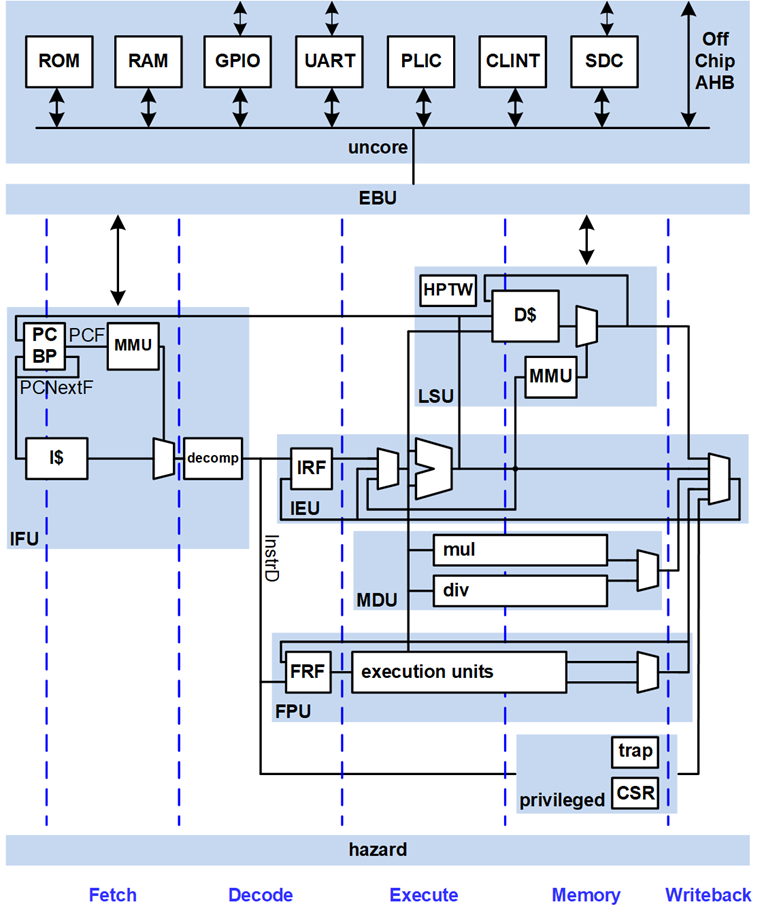
\includegraphics[width=0.9\linewidth]{WALLY_diagram.png}}
\caption{Block Diagram of the WALLY system [1]}
\label{fig}
\end{figure}

The primary goal is to achieve significant power efficiency, specifically targeting a 30\% reduction in system power. This will be accomplished through systematic architectural and implementation-level power optimizations, culminating in a validated, energy-efficient processor.

\section{Methods}

This project will be broken across two semesters, and thus I designed a set of goals for each semester. This semester, the goals are to set up a Virtual Machine with all the needed tools for design and verification, build the base WALLY design on an FPGA and run benchmark tests, and create a set of design specifications for the final design. This will allow me to work on more physical design aspects next semester.

For this semester, the work will be done using a Virtual Machine on the Rice ORION cluster. This will include validating the existing design, and modifying the source RTL to use the proper extensions. This will also require discussion into the desired extension set. I will also use Questa and Verilator as simulation tools to test each set of extensions on the design.

\section{Results}

\subsection{Development Environment Setup}

The initial work in developing WALLY requires a reliable development environment. For this purpose, I set up a Virtual Machine (VM) on the ORION system. This setup is complete, and I am able to see the source files and run verification tests. I created an instructional document detailing the steps required to set up the WALLY project for development for future users. This process is currently undergoing testing by a senior capstone team, who is also working with WALLY. The WALLY core itself is available through an open-source GitHub repository [1].
In addition to the GitHub repository, the VM contains open-source and proprietary chip design software. This includes open-source RISC-V compilers, and Verilator, an open-source SystemVerilog simulator. It also includes Questa, Design Compiler, and Vivado, commercial chip design tools.


\subsection{WALLY on an FPGA}
In order to implement WALLY on an FPGA, I first had to decide on a specific board to use. The WALLY GitHub provides three options for FPGA implementations, but the most affordable option is the Arty A7 100T FPGA Board from Digilent. This board contains an AMD Artix-7 FPGA, as well as the needed connections for testing, including JTAG and UART support, as well as PMOD connectors that can be used to access an SD card [2].

\begin{figure}[htbp]
\centerline{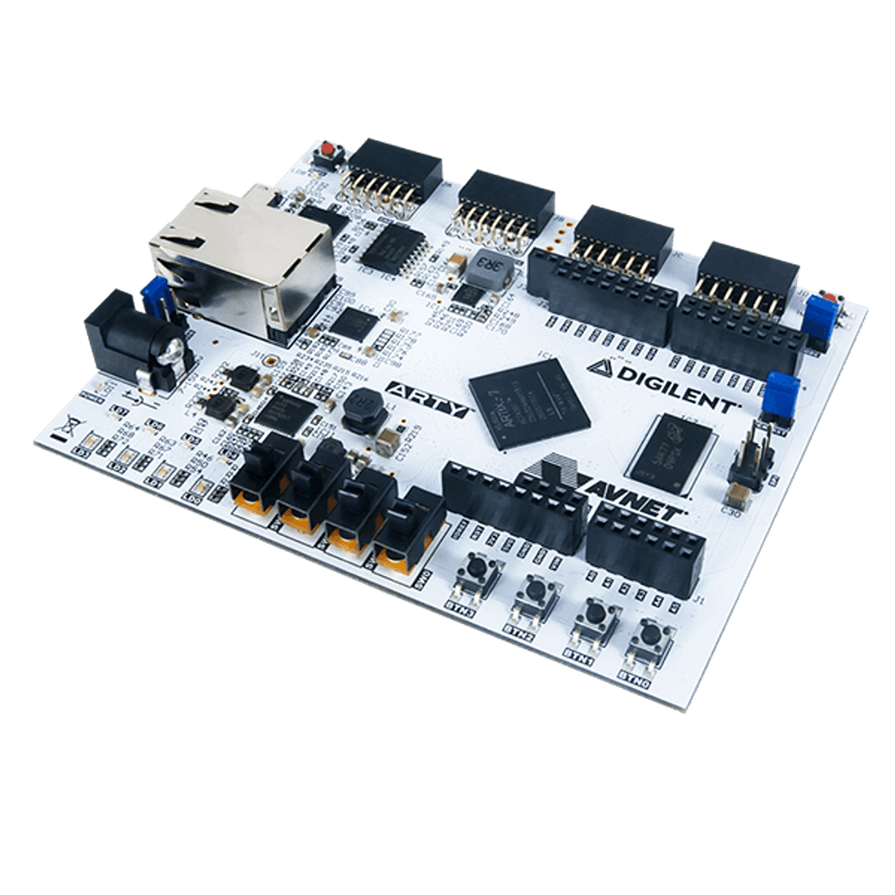
\includegraphics[width=0.9\linewidth]{Arty.png}}
\caption{The Arty A7 100-T FPGA Board [2]}
\label{fig}
\end{figure}

With this board chosen, I was able to use Vivado to generate a bitfile to program the FPGA with. The WALLY GitHub provided a script to flash an SD card with a Linux Kernel image, but since I was using a VM I could not directly flash it. So, I modified the script to write the output to a file, which I was then able to download and flash from my laptop. I also copied the Vivado project to my computer to program the FPGA.

I was able boot Linux on the FPGA, and running basic commands to demonstrate that it was responsive and functional. Screenshots showing the FPGA board booting Linux and responding to commands can be seen below.

\begin{figure}[htbp]
\centerline{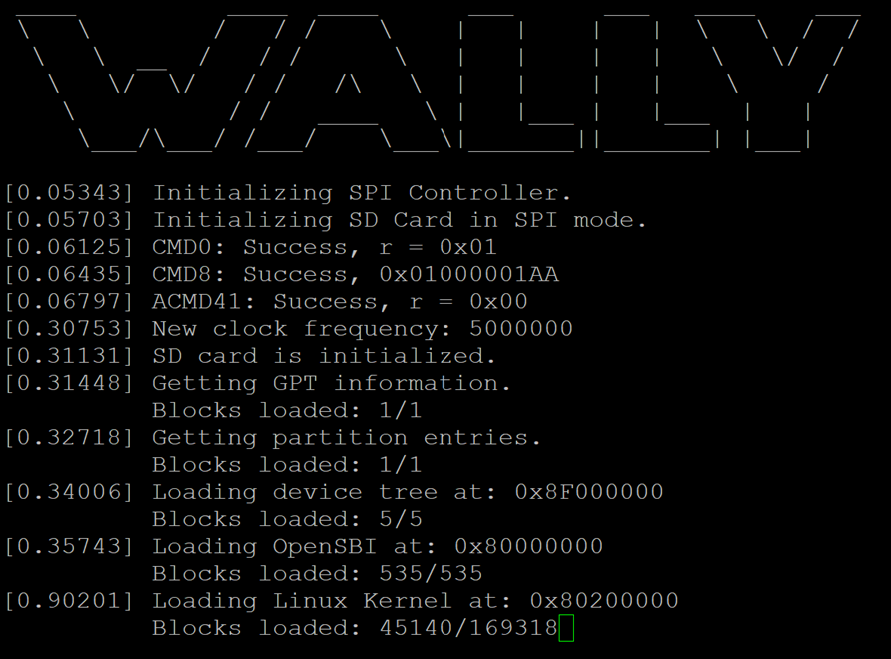
\includegraphics[width=0.9\linewidth]{Linux_Boot.png}}
\centerline{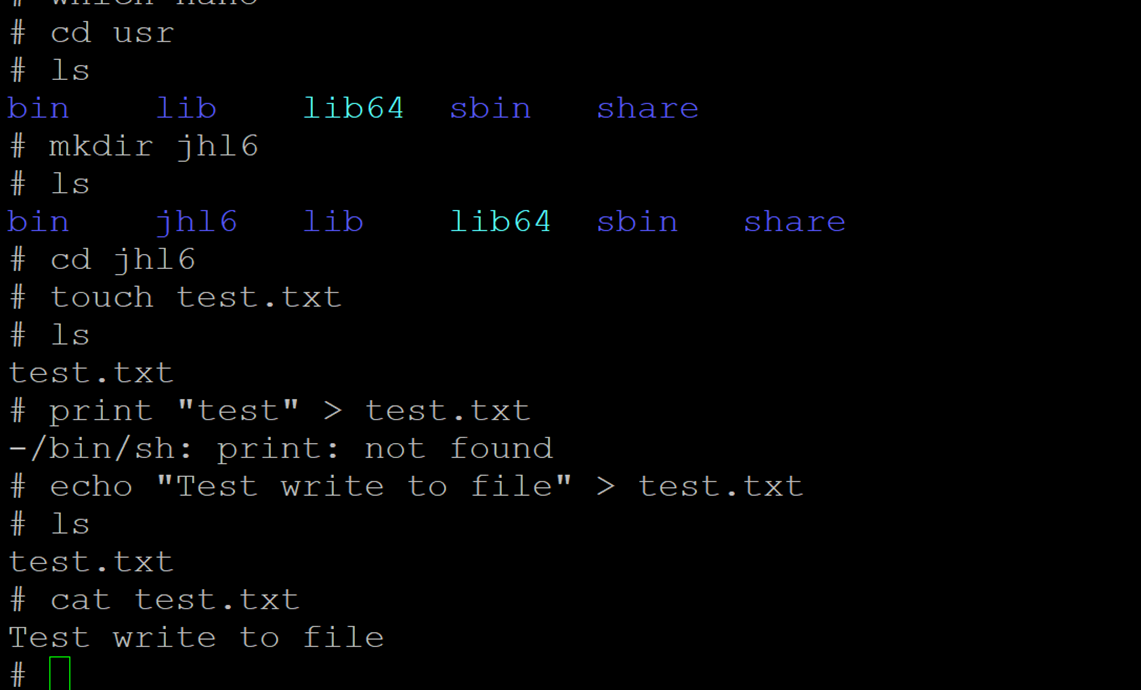
\includegraphics[width=0.9\linewidth]{WALLY_Linux.png}}
\caption{Linux Booting and Running on WALLY}
\label{fig}
\end{figure}

The next steps for this portion of the project involve deciding on a testing plan. I need to be able to test several designs and compare power usage for each, which may be done on the FPGA or in simulation.

\subsection{Design Specifications}

Our goal is to create a fully functional RISC-V processor with ultra low-power usage. In order to minimize power usage, we will need to cut down as many extensions as possible while still keeping the core functionality of the chip. To identify the most power-efficient configuration, this semester's work will focus on comparing the power usage of several design components using simulation and FPGA testing. Components under investigation include the cache configuration, the division unit, and the branch prediction logic. The results of this analysis will be used to decide on the best architectural configuration. The current design plan specifies the following features:


\begin{itemize}
    \item A \textbf{single-core, single-threaded processor}.
    \item An \textbf{integer-only} instruction set.
    \item Inclusion of the \textbf{base instruction set}.
    \item Inclusion of the \textbf{compressed (C)} instruction set to reduce code memory usage.
    \item Inclusion of the \textbf{minimal multiplication (Zmmul)} extension. This implements multiplication but not division, allowing for increased performance while avoiding the full area requirement of division circuitry.
\end{itemize}

The design specification for the SPARK-V core maintains a high degree of flexibility, prioritizing power efficiency while allowing for targeted performance enhancements. Additional components, such as a dedicated division unit or an instruction/data cache, may be incorporated if testing determines their benefits outweigh the marginal power cost. The decision to include a division unit, for instance, will depend on whether its performance gain in critical biomedical signal processing routines justifies the increased complexity and area overhead, especially since multiplication is already included. Similarly, the incorporation of a cache will be evaluated by comparing its power consumption against the energy savings achieved by reducing external memory accesses. This iterative process, which involves comparing the power usage of several different designs, ensures that the final architecture remains energy-conscious. Therefore, the core will only adopt new extensions or subsystems that offer a substantial, application-specific return on investment in terms of power-to-performance ratio. This also means that future testing will require some examples of programs and routines that are common in biomedical sensors, so that functional unit usage can be measured.

In addition to these decisions that affect the core of WALLY, I also need to decide how to manage the peripheral connections WALLY contains. As per the GitHub project, these components are referred to as the "uncore" module. These include ROM, RAM, timers, GPIO, and communication over UART. While the design of the core has been specified above, additonal work will be needed to decide which uncore components will be used, and what settings will be applied to them.

\section{Discussion}
At this point in the semester, I have been able to set up the needed development environment on ORION and validate the base WALLY design by using it to boot Linux on an FPGA. I also defined an initial architectural specification with the goal of maximizing power-efficiency for wearable biomedical applications. This plan focuses on a minimalist design through the reduction of extensions and add-ons. The current specification is a single-core, single-threaded, integer-only processor utilizing the base instruction set, the compressed (C) extension to reduce code size, and the multiplication (Zmmul) extension (excluding division) for performance. The next focus is to test and finalize the best architectural configuration based on the initial design specification. This will involve using simulation and FPGA testing to compare the power usage of key design elements, such as caches, division unit implementation, and branch prediction.

Looking ahead to next semester, the project will move into the physical design phase. The primary goal is to start from the optimized architectural configuration and apply implementation-level decisions to achieve the overall objective of a 30\% reduction in system power. Ultimately, the aim is to produce a validated, energy-efficient processor ready for tapeout. I am also looking into additional power-reduction possibilities, including a paper that proposes an entirely battery-less RISC-V processor, which would be an extremely interesting implementation if possible with this design [3]. This could allow for a truly mobile processor for medical applications, but may introduce new challenges.

\section*{Acknowledgment}

I would like to thank Dr. Ray Simar for his support on this project, as well as Dr. James Stine and Jacob Pease from Oklahoma State University for their continued guidance. I would also like to thank David Harris and Sarah Harris for granting pre-publication access to their textbook covering the WALLY design which has helped in understanding the processor. Additionally, thanks to the Rice Electrical and Computer Engineering Department for funding this project.

\section*{CRediT Author Statement}
\textbf{Justin Lebeau:}
Conceptualization, Investigation, Methodology, Software, Validation, Writing

\begin{thebibliography}{00}
\bibitem{b1} https://github.com/openhwgroup/cvw
\bibitem{b2} https://digilent.com/shop/arty-a7-100t-artix-7-fpga-development-board/
\bibitem{b3} D. S. Truesdell, J. Breiholz, S. Kamineni, N. Liu, A. Magyar and B. H. Calhoun, "A 6–140-nW 11 Hz–8.2-kHz DVFS RISC-V Microprocessor Using Scalable Dynamic Leakage-Suppression Logic," in IEEE Solid-State
Circuits Letters, vol. 2, no. 8, pp. 57-60, Aug. 2019, doi: 10.1109/LSSC.2019.2938897.

\end{thebibliography}

\end{document}
